\documentclass{report}

\input{preamble}
\input{macros}
\input{letterfonts}

\title{\Huge{Math 244}}
\author{\huge{PSET 3}}
\date{Feb 10 2025}

\begin{document}

% Define some pastel colors
\definecolor{pastelPink}{HTML}{ffb3ba}     % "#ffb3ba"
\definecolor{pastelBlue}{HTML}{b3cde0}     % "#b3cde0"
\definecolor{pastelGreen}{HTML}{ccebc5}    % "#ccebc5"
\definecolor{pastelLavender}{HTML}{c6aed8} % "#c6aed8"

\maketitle
\newpage% or \cleardoublepage
% \pdfbookmark[<level>]{<title>}{<dest>}
\pdfbookmark[section]{\contentsname}{toc}
\tableofcontents
\pagebreak

\section*{2.3 Prob 1}
\addcontentsline{toc}{section}{Prob 1}

\qs{}{
  How many linear extensions of $\mathcal{B}_2$ are there, and what about $\mathcal{B}_3$?
}



\begin{center}
  \begin{tikzpicture}[scale=1.0, 
      every node/.style={circle, draw, thick, minimum size=10mm, inner sep=0pt, font=\footnotesize}]
      
    % First lattice: B2 on the left
    \node (topB2) at (-4,1.5) [fill=pastelPink] {\(\{a,b\}\)};
    \node (aB2)   at (-5,0)   [fill=pastelBlue] {\(\{a\}\)};
    \node (bB2)   at (-3,0)   [fill=pastelBlue] {\(\{b\}\)};
    \node (botB2) at (-4,-1.5) [fill=pastelLavender] {\(\varnothing\)};

    % -- B2 edges --
    \draw[thick] (topB2) -- (aB2);
    \draw[thick] (topB2) -- (bB2);
    \draw[thick] (aB2) -- (botB2);
    \draw[thick] (bB2) -- (botB2);

    % Label for B2
    \node[draw=none, fill=none, below=8mm] at (-4,-2.2) {\(\mathbf{B_2}\)};

    % Second lattice: B3 on the right
    \node (top) at (2,3) [fill=pastelPink]   {\(\{a,b,c\}\)};
    \node (ab)  at (0,1.5) [fill=pastelBlue]    {\(\{a,b\}\)};
    \node (ac)  at (2,1.5) [fill=pastelBlue]    {\(\{a,c\}\)};
    \node (bc)  at (4,1.5) [fill=pastelBlue]    {\(\{b,c\}\)};
    \node (a)   at (0,0) [fill=pastelGreen]   {\(\{a\}\)};
    \node (b)   at (2,0) [fill=pastelGreen]   {\(\{b\}\)};
    \node (c)   at (4,0) [fill=pastelGreen]   {\(\{c\}\)};
    \node (bot) at (2,-1.5) [fill=pastelLavender] {\(\varnothing\)};

    % -- B3 edges --
    \draw[thick] (top) -- (ab);
    \draw[thick] (top) -- (ac);
    \draw[thick] (top) -- (bc);

    \draw[thick] (ab) -- (a);
    \draw[thick] (ab) -- (b);
    \draw[thick] (ac) -- (a);
    \draw[thick] (ac) -- (c);
    \draw[thick] (bc) -- (b);
    \draw[thick] (bc) -- (c);

    \draw[thick] (a) -- (bot);
    \draw[thick] (b) -- (bot);
    \draw[thick] (c) -- (bot);

    % Label for B3
    \node[draw=none, fill=none, below=8mm] at (2,-2.2) {\(\mathbf{B_3}\)};
  \end{tikzpicture}
\end{center}


\begin{RemarkWithLily}{For Prob 1}
  FFor $\mathcal{B}_2$ $\varnothing$ is the unique minimal element, it must appear first in any linear extension, and $\{a,b\}$ is the unique maximal element, so it must appear last. The only freedom in ordering comes from the two singletons, $\{a\}$ and $\{b\}$, which are incomparable. There are $2! = 2$ ways to arrange these elements. Therefore, the total number of linear extensions is 
  \[
  2.
  \]

  \medskip

  For $\mathcal{B}_3$ the empty set $\varnothing$ is minimal and must come first in any linear extension.  
  Next, we must place two of the three singletons, and there are $3\times 2=6$ ways to choose and order these first two.  
  After this, there are two possibilities:
  \begin{enumerate}
  \item Place the remaining singleton next. Then the three 2-element subsets may appear in any order before the full set $\{a,b,c\}$, contributing $3!=6$ arrangements.
  \item Place the 2-element set formed by the first two singletons next. Then the remaining singleton must appear before any 2-element set containing it, so it appears immediately after, leaving 2 ways to order the remaining two 2-subsets.
  \end{enumerate}
  Hence, for each of the $6$ ways to choose the first two singletons, there are $6 + 2 = 8$ ways to continue.  The total number of linear extensions is therefore
  \[
  6 \times 8 \;=\; 48.
  \]
\end{RemarkWithLily}


\newpage 



\section*{Bonus Problem}
\addcontentsline{toc}{section}{Bonus Prob}

\qs{}{
  Prove that not every
  finite poset admits an embedding into the poset $( \mathbb{N}^2, \preceq)$, where
  $(x_1, y_1)\preceq (x_2, y_2)$ if and only if $x_1 \leq x_2$ and $y_1 \leq y_2$.
}


\begin{proofWithHibiscus}
  Suppose a finite poset $P$ can be embedded into $(\mathbb{N}^2, \preceq)$. There exists an injective function
  \[ f: P \to \mathbb{N}^2, \]
 that for all $x,y\in P$,
  \[ x \le_P y \quad \Longleftrightarrow \quad f(x) \preceq f(y), \]
  
  \[ f(x) = (x_1,x_2) \quad \text{and} \quad f(y) = (y_1,y_2)\] 

  \[ (x_1,x_2) \preceq (y_1,y_2) \quad \Longleftrightarrow \quad x_1 \le y_1 \quad \text{and} \quad x_2 \le y_2. \]

  Define two linear orders on $P$ as follows:
  \begin{enumerate}[label=\textbf{Order \arabic*:}]
      \item Define $L_1$ on $P$ by
      \[
      x \le_{L_1} y \quad \Longleftrightarrow \quad f(x)_1 \le f(y)_1.
      \]
      \item Define $L_2$ on $P$ by
      \[
      x \le_{L_2} y \quad \Longleftrightarrow \quad f(x)_2 \le f(y)_2.
      \]
  \end{enumerate}
  Since $\mathbb{N}$ is totally ordered, both $L_1$ and $L_2$ are linear (total) orders.

  We now show that the original poset order on $P$ is the intersection of these two orders. Indeed:
  \begin{itemize}
      \item If $x \le_P y$, then by the definition of the embedding, 
      \[
      f(x)_1 \le f(y)_1 \quad \text{and} \quad f(x)_2 \le f(y)_2.
      \]
      Hence, $x \le_{L_1} y$ and $x \le_{L_2} y$.
      \item Conversely, if $x \le_{L_1} y$ and $x \le_{L_2} y$, then
      \[
      f(x)_1 \le f(y)_1 \quad \text{and} \quad f(x)_2 \le f(y)_2,
      \]
      so that $f(x) \preceq f(y)$, and thus $x \le_P y$.
  \end{itemize}

  This shows that
  \[
  x \le_P y \quad \Longleftrightarrow \quad \bigl( x \le_{L_1} y \text{ and } x \le_{L_2} y \bigr).
  \]
  Therefore, the poset $P$ is the intersection of two linear orders, meaning its \emph{order dimension} is at most $2$. \\

  It is a well-known fact in order theory that there exist finite posets with order dimension greater than $2$. For example, the Boolean lattice $B_3$---the poset of all subsets of a $3$-element set ordered by inclusion---has order dimension $3$. More generally, for any integer $d \ge 1$, there exists a finite poset with order dimension $d$.\\

  Since any poset that embeds into $(\mathbb{N}^2, \preceq)$ must have order dimension at most $2$, it follows that any finite poset with order dimension greater than $2$ cannot be embedded into $(\mathbb{N}^2, \preceq)$. Therefore, not every finite poset admits an embedding into $(\mathbb{N}^2, \preceq)$.

  \[
  \boxed{\text{Not every finite poset can be embedded into } (\mathbb{N}^2, \preceq).}
  \]
\end{proofWithHibiscus}

\newpage 

\section*{2.4 Prob 3}
\addcontentsline{toc}{section}{Prob 2}

\qs{}{
  Find a sequence of real numbers of length 16 that contains no monotone
  subsequence of length 5.
}

\begin{center}
  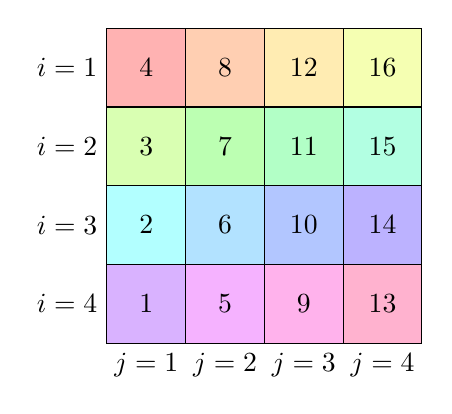
\begin{tikzpicture}[scale=1]
    % Loop over rows i=1..4 and columns j=1..4
    \foreach \i in {1,2,3,4} {%
      \foreach \j in {1,2,3,4} {%
        % Compute the value to display
        \pgfmathtruncatemacro{\val}{4*(\j-1) + (5-\i)}
        % Compute a hue between 0 and 1 depending on row and column.
        \pgfmathsetmacro{\hue}{((\i-1)*4 + (\j-1))/16}
        %
        % --- Convert HSV (hue, 0.3, 1) to RGB ---
        % Compute H' = 6 * hue.
        \pgfmathsetmacro{\Hprime}{6*\hue}
        % Determine the sector (an integer between 0 and 5)
        \pgfmathtruncatemacro{\sector}{floor(\Hprime)}
        % The fractional part
        \pgfmathsetmacro{\f}{\Hprime - \sector}
        % p is constant because saturation is 0.3:
        \pgfmathsetmacro{\pval}{0.7} % since 1 - 0.3 = 0.7
        % q and t depend on f:
        \pgfmathsetmacro{\qval}{1 - \f*0.3}
        \pgfmathsetmacro{\tval}{1 - (1-\f)*0.3}
        %
        % Now set r,g,b based on the sector.
        % We use TeX conditionals (\ifcase ... \fi). The numbers will be stored in
        % macros \rval, \gval, \bval.
        \ifcase\sector
          \def\rval{1}%
          \def\gval{\tval}%
          \def\bval{\pval}%
        \or
          \def\rval{\qval}%
          \def\gval{1}%
          \def\bval{\pval}%
        \or
          \def\rval{\pval}%
          \def\gval{1}%
          \def\bval{\tval}%
        \or
          \def\rval{\pval}%
          \def\gval{\qval}%
          \def\bval{1}%
        \or
          \def\rval{\tval}%
          \def\gval{\pval}%
          \def\bval{1}%
        \or
          \def\rval{1}%
          \def\gval{\pval}%
          \def\bval{\qval}%
        \fi
        %
        % Draw the cell using the computed RGB color.
        % The fill syntax here uses the "rgb" model.
        \node[draw,
              fill={rgb,1:red,\rval; green,\gval; blue,\bval},
              minimum width=1cm,
              minimum height=1cm]
              at (\j,-\i) {\(\val\)};
      }%
    }
    
    % Place row labels to the left (using anchor=east so they don’t touch the boxes)
    \node[anchor=east] at (0.5, -1) {\(i=1\)};
    \node[anchor=east] at (0.5, -2) {\(i=2\)};
    \node[anchor=east] at (0.5, -3) {\(i=3\)};
    \node[anchor=east] at (0.5, -4) {\(i=4\)};
    
    % Place column labels below (using anchor=north)
    \node[anchor=north] at (1, -4.5) {\(j=1\)};
    \node[anchor=north] at (2, -4.5) {\(j=2\)};
    \node[anchor=north] at (3, -4.5) {\(j=3\)};
    \node[anchor=north] at (4, -4.5) {\(j=4\)};
  \end{tikzpicture}
\end{center}

\bigskip



\exrose{For Prob 2}{
  RReading the cells row by row (from top row to bottom row) gives the sequence:
  \[
  4, 8, 12, 16,\quad
  3, 7, 11, 15,\quad
  2, 6, 10, 14,\quad
  1, 5, 9, 13.
  \]
  Why there can't be an increasing subsequence of length 5.

  \medskip

  This works because we split the sequence into a matrice of of $ 4 \times 4$ and by the pigeonhole 
  principle, if you were to pick 5 numbers from the sequence at least of them would have to come from the same column 
  but in each column, the numbers appear in decreasing order thus any two numbers comming from teh same cloum will be in decreasing 
  order which prevents the entire subsequence from being increasing. 
  \bigskip

  Why there can't be a strictly decreasing subsequence of length 5 

  \medskip
  
  A similar argument applies for the decreasing subsequence. Our grid has 4 rows and if you were to pick 5 numbers from teh sequence 
  then by the pigeonhole principle at least two would have to come from the same row 
  but the entries in each row are in increasing order preventing a nondecreasing sequence of length 5.

}


\newpage 

\section*{2.4 Prob 4}
\addcontentsline{toc}{section}{Prob 3}

\qs{}{
  Prove the following strengthening of Theorem 2.4.6: Let $k, \ell$ be
  natural numbers. Then every sequence of real numbers of length $k \ell + 1$
  contains a nondecreasing subsequence of length $k+1$ or a decreasing subsequence of
  length $ \ell +1$.
}


\begin{proofWithHibiscus}
  Let $(x_1, x_2, \ldots, x_{k\ell + 1})$ be any sequence of real numbers and let 
  \[
    X \;=\; \{\,1,2,\ldots, k\ell + 1\}.
  \]
  We define a relation $\preceq$ on $X$ by 
  \[
    i \preceq j 
    \quad\Longleftrightarrow\quad 
    i \le j 
    \;\text{ and }\;
    x_i \,\le\, x_j.
  \]
  \smallskip

  \begin{ClaimWithMagnolia}
    The relation $\preceq$ is a partial order on $X$.
    
    \medskip
    \noindent
    \emph{Proof of Claim.} 
    \begin{itemize}
      \item \textbf{Reflexivity:} 
      For every $i \in X$, we have $i \le i$ and $x_i \le x_i$. Hence $i \preceq i$.
      
      \item \textbf{Antisymmetry:} 
      Suppose $i \preceq j$ and $j \preceq i$. Then $i \le j$, $j \le i$, $x_i \le x_j$, and $x_j \le x_i$. 
      Thus $i = j$ and $x_i = x_j$, so $i \preceq j$ and $j \preceq i$ imply $i=j$.
      
      \item \textbf{Transitivity:} 
      Suppose $i \preceq j$ and $j \preceq k$. Then $i \le j \le k$ and 
      $x_i \le x_j \le x_k$. Consequently $i \le k$ and $x_i \le x_k$, so $i \preceq k$.
    \end{itemize}
    Hence $\preceq$ is indeed a partial order.
  \end{ClaimWithMagnolia}

  \medskip
  We now observe that in this poset $(X, \preceq)$:
  \begin{itemize}
    \item A \emph{chain} of size $m$ corresponds to indices 
      $i_1 < i_2 < \cdots < i_m$ such that 
      $x_{i_1} \le x_{i_2} \le \cdots \le x_{i_m}$,
    \item An \emph{antichain} of size $m$ corresponds to indices 
      $i_1 < i_2 < \cdots < i_m$ for which no two are comparable under $\preceq$, so
      $x_{i_1} > x_{i_2} > \cdots > x_{i_m}$, 
  \end{itemize}

  By Dilworth's theorem every finite poset $P=(X,\preceq)$ satisfies
  \[
    |X|\;\;\le\;\;\alpha(P)\,\cdot\,\omega(P),
  \]
  where $\alpha(P)$ is the maximum size of any antichain in $P$ and $\omega(P)$ is the maximum size of any chain. 
  Applying this to our poset $(X,\preceq)$ yields
  \[
    k\ell + 1 
    \;=\;
    |X|
    \;\;\le\;\;
    \alpha\bigl(X,\preceq\bigr)\;\cdot\;\omega\bigl(X,\preceq\bigr).
  \]
  It is impossible for both $\alpha(P) \le \ell$ and $\omega(P) \le k$ to hold, 
  since that would force 
  \(
    \alpha(P)\,\cdot\,\omega(P) \;\le\; k\ell \,<\, k\ell+1.
  \)
  Therefore, at least one of the following must be true:
  \[
    \alpha(P) \;\ge\; \ell + 1
    \qquad\text{or}\qquad
    \omega(P) \;\ge\; k + 1.
  \]
\end{proofWithHibiscus}


\section*{3.1 Prob 2}
\addcontentsline{toc}{section}{Prob 4}

\qs{}{
  Determine the number of ordered pairs $(A, B)$, where $A \subseteq B \subseteq \{ 1, 2, \ldots, n \}$.
}

\begin{proofWithHibiscus}
  Let $X = \{1,2,\ldots,n\}$. We wish to count the number of ordered pairs $(A,B)$ such that
  \[
    A \;\subseteq\; B \;\subseteq\; X.
  \]

  For each element $i \in X$, there are exactly three ways to place $i$ with respect to the pair $(A,B)$:
  \[
    \text{(1) } i \;\notin\; B\;(\text{so } i \notin A), 
    \quad 
    \text{(2) } i \;\in\; B \setminus A,
    \quad
    \text{(3) } i \;\in\; A \subseteq B.
  \]
  If we make this choice for every element $i \in X$, we determine a pair $(A,B)$ with $A \subseteq B$. 

  \medskip

  Since each of the $n$ elements admits exactly three possibilities, the total number of ordered pairs $(A,B)$ with $A \subseteq B \subseteq X$ is
  \[
    3^n.
  \]
\end{proofWithHibiscus}


\section*{3.1 Prob 6}
\addcontentsline{toc}{section}{Prob 5}

\qs{}{
  Show that a natural number $n \ge 1$ has an odd number of divisors
  (including 1 and itself) if and only if $\sqrt{n}$ is an integer. {\it The textbook
  has a hint to this problem in the back.}
}

\begin{proofWithHibiscus}
  Let $d(n)$ be the number of positive divisors of $n$ including $1$ and $n$ itself. 

  \bigskip

  (\(\Longrightarrow\))
  Suppose $d(n)$ is odd. We will show that $n$ must be a perfect square. 
  Consider the divisors of $n$. Each divisor $k$ can be paired with its fellow divisor $\tfrac{n}{k}$. 
  Normally divisors come in pairs but since $d(n)$ is odd, at least one divisor must be “self-paired,” 
  $k = \tfrac{n}{k}$. Solving $k^2 = n$ shows that $k = \sqrt{n}$ is an integer. 
  So $n$ is a perfect square.

  \bigskip

  (\(\Longleftarrow\))
  Suppose $n = m^2$ for some integer $m \ge 1$. Then each positive divisor $k \neq m$ 
  of $n$ can be paired uniquely with $n/k = \tfrac{m^2}{k} \neq k$. Only the divisor 
  $k = m$ is paired with itself. Hence all divisors except $m$ come in distinct pairs, 
  and the divisor $m$ stands alone, contributing $1$ more to the total count. 
  Therefore $d(n)$ is an odd number.

\end{proofWithHibiscus}


\end{document}